We can take the KMeans algorithm as an example.
The closed-loop learning (CLL) algorithm is iterative, with the following steps in each cycle:
\begin{itemize}
    \item Apply KMeans clustering to the dataset, obtaining a hard labeling of the points.
    \item For each cluster, compute the mean and variance; this defines a mixture of Gaussians, one Gaussian per cluster.
    \item Generate $M$ synthetic points from the Gaussian mixture defined above and add these points to the dataset.
    \item Repeat the process, with the dataset growing at each step.
\end{itemize}

For example this is what happens to a KMeans clustering of the Iris Dataset after a CLL of 200 steps with $M=20$:

\begin{figure}[H]
  \centering
  \begin{minipage}{0.49\textwidth}
    \centering
    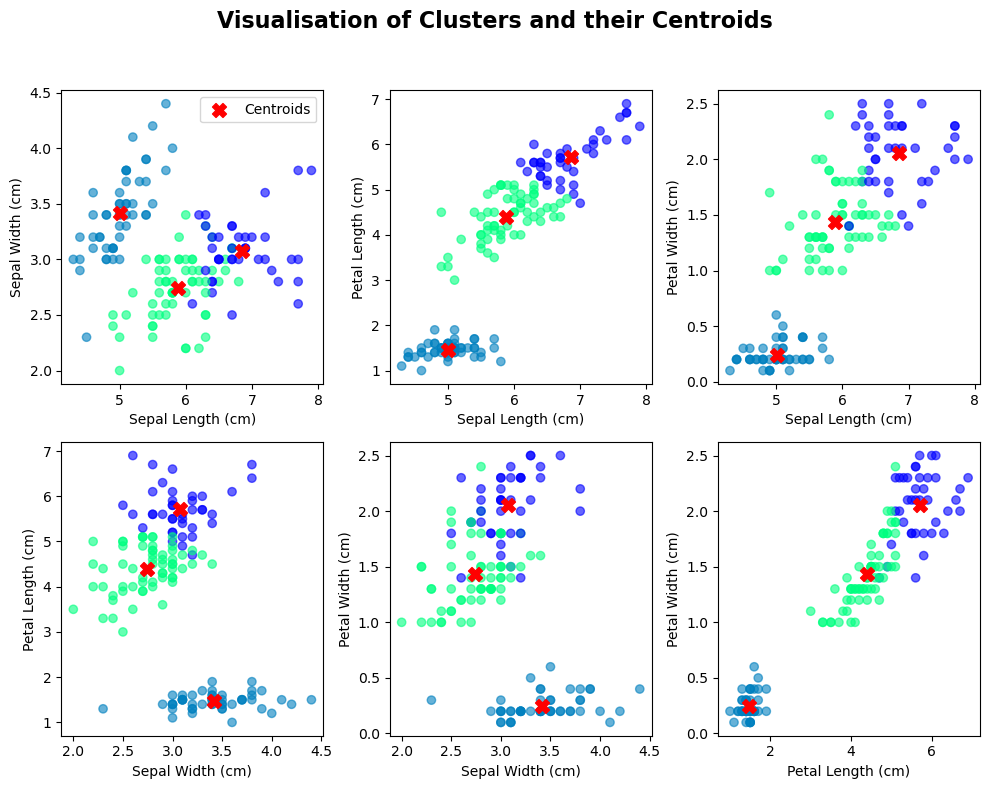
\includegraphics[width=\linewidth]{img/first_kmeans_clustering.png}
    \caption{Before CLL}
    \label{fig:iris_before}
  \end{minipage}\hfill
  \begin{minipage}{0.49\textwidth}
    \centering
    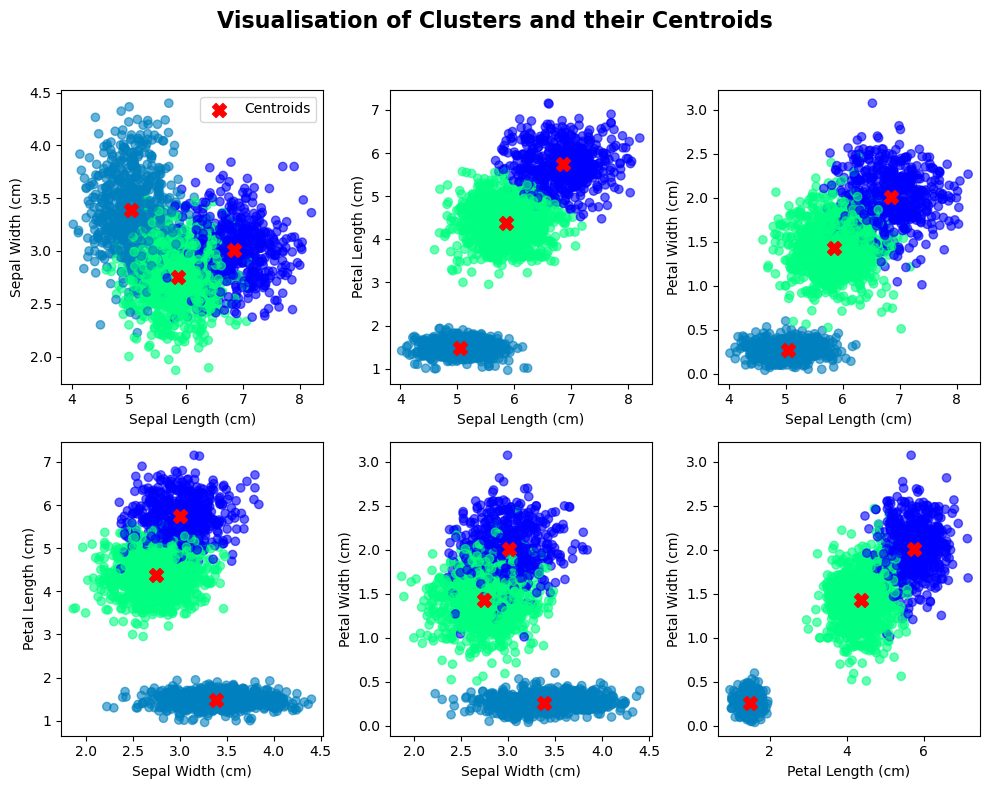
\includegraphics[width=\linewidth]{img/final_clustering.png}
    \caption{After CLL (200 steps, $M=20$)}
    \label{fig:iris_after}
  \end{minipage}
\end{figure}

We expect that, after the CLL algorithm has converged, the cluster centers will have shifted slightly. \\

Assuming that CLL is a valid, convergent clustering procedure, we can assess the quality of the original method (here KMeans) by measuring the displacements and fluctuations of the centroids.

We can plot the norm of the displacements of the centroids from initial conditions at each step of the algorithm:

\begin{figure} [H]
\centering
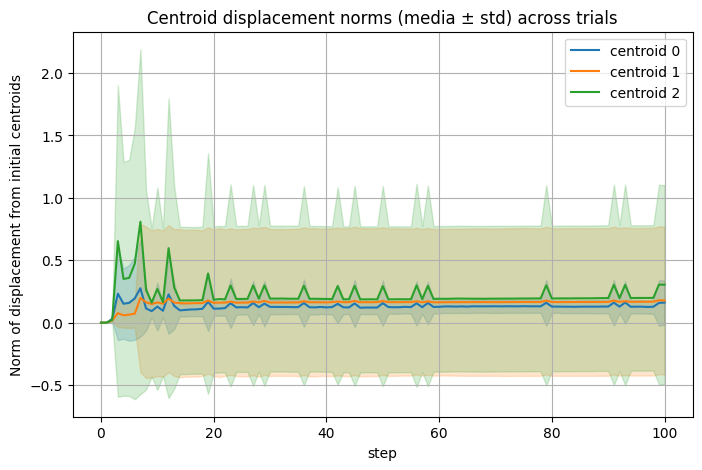
\includegraphics[width=\linewidth]{img/displacement of centroids.png}
\end{figure}

